\documentclass[11pt,oneside]{article}

	% History ================================================================
	% 2023.06.03 - Modified from Chase Murray's version
	% ========================================================================

    % STANDARD PACKAGES ======================================================
    \usepackage{datetime}
    \usepackage{graphicx}
    % \usepackage{ctex} % Allow Chinese characters
    \usepackage[utf8]{inputenc}
    \usepackage[american]{babel}
    \usepackage{amssymb}
    \usepackage[intlimits]{amsmath}
    \usepackage{amsfonts}
    \usepackage{amsthm}
    \usepackage{array}
    \usepackage{mdwlist}        
    \usepackage[labelsep=quad,indention=10pt]{subfig}
    \usepackage{algorithm}
    \usepackage[noend]{algpseudocode}
    \usepackage{lscape}
    \usepackage{rotating} % Allows \begin{sideways} \end{sideways} for vertical table headers.    
    \usepackage{threeparttable} % Allow footnotes in tables.    
    \usepackage{tabularx}
    \usepackage{multirow} % Allow table cells to span multiple rows/cols.
    \usepackage{makecell}
    \usepackage{longtable}
    \usepackage{url} % Allow \url{} and \href{url}{name}
    \usepackage{verbatim}    
    \usepackage{enumerate} % http://www.tex.ac.uk/cgi-bin/texfaq2html?label=enumerate
    \usepackage{color} % Allow colored fonts
    \usepackage[toc,page]{appendix}

    \usepackage{bm}

    \usepackage{tikz}
    \usepackage{diagbox}
    \usepackage{lastpage} % \pageref{LastPage} = total number of pages.
    \usepackage{ifthen}        
    \usepackage{setspace} % Allows \singlespacing, \onehalfspacing, \doublespacing 
    \usepackage{listings} % Allows formatting of Python code (and other languages)
    \usepackage{wrapfig}
    \usepackage[normalem]{ulem} % Allows strikethrough (\sout{text to strike})
    % \usepackage{subfigure}        % Allows subfigs/subfloats


    \usepackage{xcolor,colortbl}    % http://ctan.org/pkg/xcolor
    % \usepackage[table]{xcolor}    % https://tex.stackexchange.com/questions/50349/color-only-a-cell-of-a-table
    
    % Make sure that {color} and {xcolor} are called before mdframed
    \usepackage[framemethod=TikZ]{mdframed}    % Allows colored textbox

    \usepackage{lipsum}                     % Dummy text
    % ========================================================================

    % DEFINE PROGRAMMING FORMAT ++++++++++++++++++++++++++++++++++++++++++++++
        \lstset{language=Python}          % Set your language (you can change the language for each code-block optionally)

        \definecolor{mygreen}{rgb}{0,0.6,0}
        \definecolor{mygray}{rgb}{0.5,0.5,0.5}
        \definecolor{mymauve}{rgb}{0.58,0,0.82}

        \lstset{
          backgroundcolor=\color{gray!05!white},   % choose the background color; you must add \usepackage{color} or \usepackage{xcolor}; should come as last argument
          basicstyle=\ttfamily,                    % the size of the fonts that are used for the code
          breakatwhitespace=false,                 % sets if automatic breaks should only happen at whitespace
          breaklines=true,                         % sets automatic line breaking
          captionpos=t,                            % sets the caption-position to bottom
          commentstyle=\color{black},              % comment style
          deletekeywords={...},                    % if you want to delete keywords from the given language
          escapeinside={\%*}{*)},                  % if you want to add LaTeX within your code
          extendedchars=true,                      % lets you use non-ASCII characters; for 8-bits encodings only, does not work with UTF-8
          frame=single,                               % adds a frame around the code
          keepspaces=true,                         % keeps spaces in text, useful for keeping indentation of code (possibly needs columns=flexible)
          % keywordstyle=\color{blue},             % keyword style
          language=Python,                         % the language of the code
          morekeywords={*,...},                    % if you want to add more keywords to the set
          numbers=left,                            % where to put the line-numbers; possible values are (none, left, right)
          numbersep=5pt,                           % how far the line-numbers are from the code
          % numberstyle=\tiny\color{mygray},       % the style that is used for the line-numbers
          rulecolor=\color{black},                 % if not set, the frame-color may be changed on line-breaks within not-black text (e.g. comments (green here))
          showspaces=false,                        % show spaces everywhere adding particular underscores; it overrides 'showstringspaces'
          showstringspaces=false,                  % underline spaces within strings only
          showtabs=false,                          % show tabs within strings adding particular underscores
          stepnumber=1,                            % the step between two line-numbers. If it's 1, each line will be numbered
          % stringstyle=\color{mymauve},           % string literal style
          tabsize=4,                               % sets default tabsize to 2 spaces
          % title=\lstname,                        % show the filename of files included with \lstinputlisting; also try caption instead of title
          xleftmargin=35pt,
          xrightmargin=15pt, 
          aboveskip=0pt,
          belowskip=5pt
        }
    % ++++++++++++++++++++++++++++++++++++++++++++++++++++++++++++++++++++++++

    % DEFINE/RENEW SOME ENVIRONMENTS =========================================    
        \renewenvironment{abstract}
          {\normalfont\footnotesize
            \list{}{\labelwidth0pt
              \leftmargin20pt \rightmargin\leftmargin
              \listparindent\parindent \itemindent0pt
              \parsep0pt
              \let\fullwidthdisplay\relax
            }
            \item[\hskip\labelsep\bfseries\abstractname:] %
        }{
          \endlist}

        \newcommand{\keywordsname}{Keywords}
        \newenvironment{keywords}
          {\normalfont\footnotesize
            \list{}{\labelwidth0pt
              \leftmargin20pt \rightmargin\leftmargin
              \listparindent\parindent \itemindent0pt
              \parsep0pt
              \let\fullwidthdisplay\relax}
            \item[\hskip\labelsep\bfseries\keywordsname:]}{\endlist}

        \newcommand{\dochistname}{History}
        \newenvironment{DocHistory}
          {\normalfont\footnotesize
            \list{}{\labelwidth0pt
              \leftmargin20pt \rightmargin\leftmargin
              \listparindent\parindent \itemindent0pt
              \parsep0pt
              \let\fullwidthdisplay\relax}
            \item[\hskip\labelsep\bfseries\dochistname:]}{\endlist}
    % ========================================================================    

    % DEFINE PAGE FORMATTING +++++++++++++++++++++++++++++++++++++++++++++++++
        % Select Line Spacing:
        \singlespacing
        % \onehalfspacing        
        % \doublespacing    

        % Margins:
        \usepackage[letterpaper,left=1.0in,top=1.0in,right=1.0in,bottom=1.0in]{geometry}
    
        % Page Style
        \pagestyle{plain}    % Includes page number
        %\pagestyle{empty}    % Completely blank                

        % By default all math is set to inline mode. The \displaystyle command
        % ensures that we don't get small fractions or summations with limits
        % on the sides.
        \everymath{\displaystyle}    
        
        % http://tex.stackexchange.com/questions/5223/command-for-argmin-or-argmax
        \DeclareMathOperator*{\argmin}{arg\,min}

        % Allow flalign items to be split over multiple pages:
        \allowdisplaybreaks[1]   % See ftp://ftp.ams.org/pub/tex/doc/amsmath/amsldoc.pdf    
    % ++++++++++++++++++++++++++++++++++++++++++++++++++++++++++++++++++++++++

    % DEFINITION, THEOREM, AND LEMMA +++++++++++++++++++++++++++++++++++++++++

        \theoremstyle{definition}
            \newtheorem{definition}{Definition}[section]
            \newtheorem*{example}{Example}
            \newtheorem{problem}{Problem}[section]
            \newtheorem*{solution}{Solution}
            \newtheorem{hypothesis}{Hypothesis}[section]
        \theoremstyle{plain}
            \newtheorem{theorem}{Theorem}[section]
            \newtheorem{corollary}{Corollary}[theorem]
            \newtheorem{lemma}[theorem]{Lemma}
            \newtheorem{conjecture}{Conjecture}
            \newtheorem{proposition}{Proposition}
        \theoremstyle{remark}
            \newtheorem*{remark}{Remark}

    % ++++++++++++++++++++++++++++++++++++++++++++++++++++++++++++++++++++++++

    % CUSTOM MACROS ++++++++++++++++++++++++++++++++++++++++++++++++++++++++++

        % This is how you may create a new variable:
        % \newcommand{\docjunk}{ text to display }
        
        % See https://gist.github.com/benkehoe/c46647134d4bbd514869
        % for more examples.

        % Create a box marked ``To Do'' around text.
        % \todo{  insert text here  }.
        \newcommand{\todo}[1]{\vspace{5 mm}\par \noindent
        \marginpar{\textsc{to do}}
        \framebox{\begin{minipage}[c]{0.95 \textwidth}
        \tt\begin{center} #1 \end{center}\end{minipage}}\vspace{5 mm}\par}

        % Create an empty box marked ``Result'' in the margin.
        % Specify the number of empty rows.
        % \result{8 em}.
        \newcommand{\result}[1]{\vspace{5 mm}\par \noindent
        \marginpar{\textsc{Result}} $\qquad\qquad$
        \framebox{\begin{minipage}[c]{0.75 \textwidth}
        \tt\begin{center} \vspace{#1} \end{center}\end{minipage}}\vspace{5 mm}\par}

        % Color selected text in red font.
        % \alert{text to color}
        \newcommand{\alert}[1]{{\color{red}#1}}

        % Color selected text in blue font.
        % \edited{text to color}
        \newcommand{\edited}[1]{{\color{blue}#1}}

        % Color selected text and add a "FIXME" note in the margin.
        % \fixme{text to color}
        \newcommand{\fixme}[1]{{\color{red}#1}
            \marginpar{\textsc{\color{red}fixme}}}

        % Color selected text (optional) and add a note in brackets.
        % \note[selected text]{comments}
        % \note{comments}
        \renewcommand{\note}[2][]{
            {\color{blue}#1 %
            [\textsc{note}:~#2]}
        }
        
        % Color selected text (optional) and add a note from someone.
        % \notefrom[selected text]{from}{comments}
        % \notefrom{from}{comments}
        \newcommand{\notefrom}[3][]{
            {\color{green!50!black}#1 %
            [\textsc{from #2}:~#3]}
        }
        
        % Color selected text (optional) and add a note to someone.
        % \noteto[selected text]{to}{comments}
        % \noteto{to}{comments}
        \newcommand{\noteto}[3][]{
            {\color{red}#1 %
            [\textsc{to #2}:~#3]}
        }

        % Color and Line Settings for Boxed Text
        \mdfsetup{
        % middlelinecolor=red,
        middlelinewidth=1pt,
        % linecolor=blue,
        % linewidth=1pt,
        backgroundcolor=orange!10!white,
        linecolor=orange!50!black,
        roundcorner=5pt}
        
        % Shortcut for referencing figures/tables:
        % Usage:  \figref{fig:name} --> Figure 1.
        \newcommand{\figref}[1]{\figurename~\ref{#1}}
        \newcommand{\tabref}[1]{\tablename~\ref{#1}}
    % ++++++++++++++++++++++++++++++++++++++++++++++++++++++++++++++++++++++++

    % SETUP TikZ +++++++++++++++++++++++++++++++++++++++++++++++++++++++++++++
        \usetikzlibrary{arrows,shapes,matrix}
        \usetikzlibrary{decorations.pathmorphing} 
        \usepgflibrary{plotmarks}
        \usetikzlibrary{patterns}  
        \usetikzlibrary{positioning} 
        \usetikzlibrary{snakes}  
        \tikzstyle{block}=[draw opacity=0.7,line width=1.4cm]
        
        % MORE STUFF TO ADD HERE?
    % ++++++++++++++++++++++++++++++++++++++++++++++++++++++++++++++++++++++++

    % SETUP BIBLIOGRAPHY +++++++++++++++++++++++++++++++++++++++++++++++++++++
    % [This section MUST be used if you have a bibliography.    ]
    % [Otherwise, leave this section commented out.        ]
    % \begin{comment}

        % FIXME -- EXPLAIN
        
        % Setup the Bibliography Style -- Select ONE of the following:
        % \usepackage{natbib}
        % \usepackage[sectionbib,square]{natbib}     %%% See natbib.pdf for explanation.
        % \usepackage[sectionbib,round]{natbib}
        \usepackage[square,numbers]{natbib}

        \bibliographystyle{plainnat}

        % Natbib setup for author-year style
        % \bibpunct has 1 optional and 6 mandatory arguments:
        %  [0.] The character preceding a post-note, default is a comma plus space. In redefining this character, 
        %     one must include a space if one is wanted. 
        %  1. the opening bracket symbol, default = (
        %  2. the closing bracket symbol, default = )
        %  3. the punctuation between multiple citations, default = ;
        %  4. the letter `n' for numerical style, or `s' for numerical superscript style, 
        %    any other letter for author-year, default = author-year;
        %  5. the punctuation that comes between the author names and the year
        %  6. the punctuation that comes between years or numbers when common author lists are suppressed (default = ,);

        % Natbib setup for author-year style
        \bibpunct[, ]{(}{)}{,}{a}{}{,}                % Use author names
        % \bibpunct[, ]{[}{]}{,}{n}{}{,}            % Use numbers
        
        \def\bibfont{\small}
        \def\bibsep{\smallskipamount}
        \def\bibhang{24pt}
        \def\newblock{\ }
        \def\BIBand{and}
    % \end{comment}
    % ++++++++++++++++++++++++++++++++++++++++++++++++++++++++++++++++++++++++

    % DOCUMENT INFO ++++++++++++++++++++++++++++++++++++++++++++++++++++++++++
        \newcommand{\docTitle}{}

        % List authors here, separated by \and 
        \newcommand{\docAuthor}{}
        % \newcommand{\docAuthor}{}

        \newcommand{\docAffil}{
            School of Management, Shanghai University, Shanghai, China
        }

        \newcommand{\docAbstract}{}

        \newcommand{\docKeyword}{}

        % This date will appear under the title.
        \newcommand{\docDate}{\today}       % {} --> don't show a date.
            
        % This date will appear in the page header:
        \newcommand{\draftDate}{\today}    % {\today} --> draft, {} --> finalized (hidden)
    
        % The image files should be saved here:
        \graphicspath{ {../../image/} }
    % ++++++++++++++++++++++++++++++++++++++++++++++++++++++++++++++++++++++++

    % DEFINE HEADER ++++++++++++++++++++++++++++++++++++++++++++++++++++++++++
        \usepackage{fancyhdr}
        \pagestyle{fancy}
        \ifthenelse{\equal{\draftDate}{}}
            {
                % This is the final version...remove the date from the header
                \chead{}
            }
            {
                % This is a working draft...include the date in the header
                % \chead{\color{red}DRAFT -- Updated \draftDate~at~\currenttime}
            }
        \lhead{}    % no left/right header content
        \rhead{}
        %\cfoot{}
        %\lfoot{}
        %\rfoot{}
        \renewcommand{\headrulewidth}{0pt}
        \renewcommand{\footrulewidth}{0pt}
        %\fancyfoot{}
    % ++++++++++++++++++++++++++++++++++++++++++++++++++++++++++++++++++++++++
    
    % DEFINE PROGRAMMING FORMAT ++++++++++++++++++++++++++++++++++++++++++++++
    \lstset{language=Python}          % Set your language (you can change the language for each code-block optionally)

    \definecolor{mygreen}{rgb}{0,0.6,0}
    \definecolor{mygray}{rgb}{0.5,0.5,0.5}
    \definecolor{mymauve}{rgb}{0.58,0,0.82}

    \lstset{ %
      backgroundcolor=\color{gray!05!white},   % choose the background color; you must add \usepackage{color} or \usepackage{xcolor}; should come as last argument
      basicstyle=\ttfamily,        % the size of the fonts that are used for the code
      breakatwhitespace=false,         % sets if automatic breaks should only happen at whitespace
      breaklines=true,                 % sets automatic line breaking
      captionpos=t,                    % sets the caption-position to bottom
      commentstyle=\color{black},    % comment style
      deletekeywords={...},            % if you want to delete keywords from the given language
      escapeinside={\%*}{*)},          % if you want to add LaTeX within your code
      extendedchars=true,              % lets you use non-ASCII characters; for 8-bits encodings only, does not work with UTF-8
      frame=single,                       % adds a frame around the code
      keepspaces=true,                 % keeps spaces in text, useful for keeping indentation of code (possibly needs columns=flexible)
      % keywordstyle=\color{blue},       % keyword style
      language=Python,                 % the language of the code
      morekeywords={*,...},           % if you want to add more keywords to the set
      numbers=none,                    % where to put the line-numbers; possible values are (none, left, right)
      numbersep=5pt,                   % how far the line-numbers are from the code
      % numberstyle=\tiny\color{mygray}, % the style that is used for the line-numbers
      rulecolor=\color{black},         % if not set, the frame-color may be changed on line-breaks within not-black text (e.g. comments (green here))
      showspaces=false,                % show spaces everywhere adding particular underscores; it overrides 'showstringspaces'
      showstringspaces=false,          % underline spaces within strings only
      showtabs=false,                  % show tabs within strings adding particular underscores
      stepnumber=1,                    % the step between two line-numbers. If it's 1, each line will be numbered
      % stringstyle=\color{mymauve},     % string literal style
      tabsize=4,                       % sets default tabsize to 2 spaces
      % title=\lstname,                   % show the filename of files included with \lstinputlisting; also try caption instead of title
      xleftmargin=35pt,
      xrightmargin=15pt, 
      aboveskip=0pt,
      belowskip=5pt
    }
    % ++++++++++++++++++++++++++++++++++++++++++++++++++++++++++++++++++++++++

    \newcommand{\titleSec}{
        % See https://tex.stackexchange.com/questions/216098/redefine-maketitle
        \begin{center}
        % \let \footnote \thanks
        {\Large \textbf{\docTitle} \par}

        % Authors?
        % Comment these lines out if you want to hide authors
        \vskip 1.0em%
        \lineskip .5em%
        \begin{tabular}[t]{c}
            \docAuthor
        \end{tabular}\par%

        % Affiliation?
        % Comment these lines out if you want to hide affiliation info
        \vskip 1.0em%
        {\small \docAffil \par}

        % Displayed date?
        % Comment these lines out if you want to hide the date
        %\vskip 1.0em%
        %{\small \docDate \par}  

        \end{center}
        \par
        \vskip 1.5em

        % \begin{abstract}
        %     \docAbstract
        % \end{abstract}

        % \begin{keywords}
        %     \docKeyword
        % \end{keywords}

        % This is version \texttt{\templateVersion} of this template.
        % Visit \templatesURL for the latest versions.
    }
\usepackage{makecell}
\setlength{\parindent}{0pt}
\usepackage{float}

\usetikzlibrary{shapes.geometric, arrows}
    \tikzstyle{startstop} = [rectangle, rounded corners, minimum width=3cm, minimum height=1cm,text centered, draw=black]
    \tikzstyle{io} = [trapezium, trapezium left angle=70, trapezium right angle=110, minimum width=3cm, minimum height=1cm, text centered, draw=black]
    \tikzstyle{process} = [rectangle, minimum width=2cm, minimum height=1cm, text centered, draw=black, inner sep=0.1cm]
    \tikzstyle{decision} = [diamond, minimum width=2cm, minimum height=0cm, text centered, draw=black, inner sep=0cm]
    \tikzstyle{arrow} = [thick,->,>=stealth]
    \tikzstyle{branchnode} = [circle, minimum size = 1cm, text centered, draw=black, inner sep=0.1cm]

\renewcommand{\docTitle}{Lecture 3 - Branch and Bound}
\renewcommand{\docAuthor}{Lan Peng, Ph.D.}
\renewcommand{\docAffil}{School of Management, Shanghai University, Shanghai, China}
\begin{document}
    \titleSec

    \begin{center}
        \textit{``The time to relax is when you don't have time for it.''}
    \end{center}

    \section{Preliminary}
        \subsection{Why Rounding Can be Bad - IP Example}
            Rounding can be bad because the optimal of IP can be far away from optimal of LP. For example,
            \begin{align*}
                \text{max} \quad & z=x_1 +0.64x_2  \\
                \text{s.t.} \quad & 50x_1 +31x_2 \le 250  \\
                            & 3x_1-2x_2\ge -4  \\
                            & x_1,x_2\ge 0 \quad \text{(for LP)}\\
                            & x_1,x_2 \in Z^+ \quad \text{(for IP)} 
            \end{align*}
            \begin{figure}[H]
                \centering
                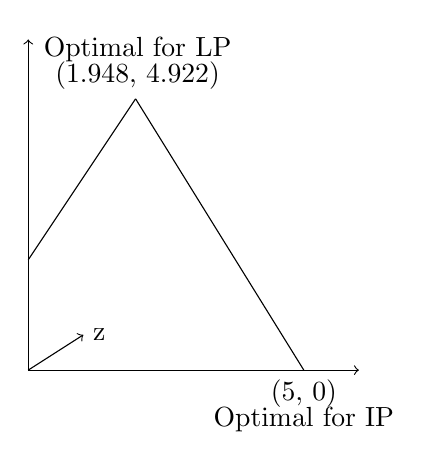
\begin{tikzpicture}[scale=0.7]
                    \draw [->] (1,1) -- (1, 7);
                    \draw [->] (1,1) -- (7, 1);
                    \draw (1,3) -- (2.948, 5.922);
                    \draw (2.948, 5.922) -- (6, 1);
                    \draw [->] (1,1) -- (2, 1.64);
                    \node [right] at (2, 1.64) {z};
                    \node [above] at (2.984, 5.922) {(1.948, 4.922)};
                    \node [above] at (2.984, 6.422) {Optimal for LP};
                    \node [below] at (6,1) {(5, 0)};
                    \node [below] at (6, 0.5) {Optimal for IP};
                \end{tikzpicture}
                \caption{Optimal solution for LP / IP}
            \end{figure}

        \subsection{Why Rounding Can be Bad - QAP example}
            Rounding can make the LP useless. For example, for QAP problem, the IP model is
            \begin{align*}
                \text{min} \quad z &= \sum_{i\in D} \sum_{s\in O} c_{is} x_{is} + \sum_{i\in D} \sum_{j \in D} \sum_{s \in O} \sum_{t\in O} w_{ij}^{st}y_{ij}^{st}  \\
                \text{s.t.} \quad & \sum_{i \in D} x_{is} =1, \quad s\in O  \\
                            &\sum_{s \in O} x_{is} = 1, \quad i \in D  \\
                            &x_{is} \in \{0, 1\}, \quad i \in D, s\in O  \\
                            & y_{ij}^{st} \ge x_{is} + x_{jt} - 1, \quad i\in D, j\in D, s\in O, t \in O  \\
                            & y_{ij}^{st} \ge 0, \quad i\in D, j\in D, s\in O, t \in O  \\
                            & y_{ij}^{st} \le x_{is}, \quad i\in D, j\in D, s\in O, t \in O  \\
                            & y_{ij}^{st} \le x_{jt}, \quad i\in D, j\in D, s\in O, t \in O  
            \end{align*}
            We can get the optimal solution for LP supposing $\forall i, s \quad x_{is}\in [0, 1]$
            \begin{align*}
                x_{is} &= \frac{1}{|D|}, \quad i \in D, s\in O   \\
                y_{ij}^{st} & = 0, \quad i\in D, j\in D, s\in O, t \in O 
            \end{align*}
           
        \subsection{Relaxation}

            \paragraph{Local Optimal v.s. Global Optimal}
                Let 
                \begin{align*}
                    Z_s &= \text{min} \{f(x):x\in S\} \\
                    Z_t &= \text{min} \{f(x):x\in T\}  \\
                    & S \subset T 
                \end{align*}
                then

                \begin{equation*}Z_t \le Z_s  \end{equation*}
                Notice that if $x_T^* \in S$ then $x_S^*=x_T^*$, to generalized it, We have

                \begin{align*}
                    \begin{cases}x_T^* \in \text{arg min} \{f(x): x\in T\} \\ x_T^* \in S\end{cases} \\ \Rightarrow x_T^*\in \text{arg min} \{f(x): x\in S\} 
                \end{align*}

                Especially for IP, we can take the LP relaxation as $T$ and the original feasible region of IP as $S$, therefore, if we find an optimal solution from LP relaxation $T$ which is also a feasible solution of $S$, then it is the optimal solution for IP ($S$)
                
            \paragraph{LP Relaxation}
                To perform the LP relaxation, we expand the feasible region
                \begin{align*}
                    x \in \{0,1\} & \rightarrow x\in [0, 1]  \\
                    y\in Z^+ & \rightarrow y \ge 0 
                \end{align*}
                If we have $Z_{LP}(s) = conv(s)$ then
                \begin{equation*} LP(s): {x\in R_+^n: Ax\le b}\end{equation*}
                The closer $LP(s)$ is to $conv(s)$ the better. Interestingly, we only need to know the convex in the direction of $c$.\\

                For IP problem
                \begin{align*}
                    Z_{IP} \quad \text{max} \quad &z = cx  \\
                            \text{s.t.} &Ax \le b \\
                                    &x\in {Z^n} 
                \end{align*}

                In feasible region $S = \{x\in Z^n, Ax\le b\}$ , the optimal solution $Z_{IP} = \text{max}\{cx: x\in S\}$. Denote $conv(S)$ as the convex hull of $S$ then

                \begin{equation*}Z_{IP}(S) = Z_{IP}(conv(S))  \end{equation*}
        
            \paragraph{Relation Between LP Relaxation and IP}
                Let
                \begin{align*}
                    Z_{IP} &=\max_{x\in S} cx, \quad \text{where } s \text{ is a set of integer solutions} \\
                    Z_{LP} &=\max cx, \quad \text{the LP relaxation of IP}  
                \end{align*}
                then
                \begin{align*}
                    Z_{IP} &= \max_{1\le i \le k} \{\max_{x \in S_i} cx \} \\
                    \text{iff} \quad S&=\bigcup_{1\le i \le k} S_i 
                \end{align*}
                Notice that $S_i$ don\rq{}t need to be disjointed.
                
            \paragraph{LP feasibility and IP(or MIP) feasibility}
                Solve the LP relaxation, one of the following things can happen
                \begin{itemize}
                    \item LP relaxation is infeasible $\rightarrow$ MIP is infeasible
                    \item LP relaxation is unbounded $\rightarrow$ MIP is infeasible or unbounded
                    \item LP relaxation has optimal solution $\hat{x}$ and $\hat{x}$ are integer ($\hat{x} \in S$), $\rightarrow$ $Z_{IP} = Z_{LP}$
                    \item LP relaxation has optimal solution $\hat{x}$ and $\hat{x}$ are not integer ($\hat{x} \notin S$), now defines a new upper bound, $Z_{LP} \ge Z_{IP}$                    
                \end{itemize}
                If the first three happens, stop, if the fourth happens, we branch and recursively solve the sub-problems.

    \section{Branch and Bound}

        \subsection{Algorithm overview}
            \begin{algorithm}[H]
                \caption{Branch and Bound (For maximization problem)}
                \begin{algorithmic}[1]
                    \State find a feasible solution as the initial Lower bound $L$
                    \State put the original LP relaxation in candidate list $S$
                    \While {$S \ne \emptyset$}
                        \State select a problem $\hat{S}$ from $S$
                        \State solve the LP relaxation of $\hat{S}$ to obtain $u(\hat{S})$
                        \If {LP is infeasible}
                            \State $\hat{S}$ pruned by infeasibility
                        \ElsIf {LP is unbounded}
                            \State \Return Unbounded
                        \ElsIf{LP $u(\hat{S}) \le L$}
                            \State $\hat{S}$ pruned by bound
                        \ElsIf{LP $u(\hat{S}) > L$}
                            \If {$\hat{x}\in S$}
                                \State $u(\hat{S})$ becomes new $L$, $L=u(\hat{S})$
                            \ElsIf {$\hat{x}\notin S$}
                                \State branch and add the new sub-problems to $S$
                                \If {LP $u(\hat{S})$ is at current best upper bound}
                                    \State set $U=u(\hat{S})$
                                \EndIf
                            \EndIf
                        \EndIf
                    \EndWhile
                    \If {Lower bound exists}
                        \State find the optimal at $L$
                    \Else
                        \State Infeasible
                    \EndIf
                \end{algorithmic}
            \end{algorithm}

        \subsection{Idea of Divide and Conquer}
            For each iteration, divide the feasible region of LP into two parts (and an infeasible part), solve the LP in those parts.\\
            \begin{figure}[H]
                \centering
                \begin{tikzpicture}[scale=0.5]
                    \draw [<->] (10, 0) -- (0,0) -- (0,10);
                    \draw (0, 8.5) -- (10, 2.5);
                    \draw (2, 8) -- (9, 0);
                    \draw [dashed] (3,0) -- (3,10);
                    \draw [dashed] (4,0) -- (4,10);
                    \node at (1.5, 5) {$S_1$};
                    \node at (3.5, 4) {$S_2$};
                    \node at (5, 3) {$S_3$}; 
                \end{tikzpicture}
                \caption{Divide and Conquer}
            \end{figure}
            In this iteration, the original feasible region have been partition into three parts, where $S_2$ is infeasible for IP because there is not integer point in it. We continue the iteration for $S_1$ and $S_2$. Each partition is suppose to give a new upper bound / lower bound and reduce the infeasible space.

            If the temp optimal integer in $S_1$ is larger than the LP relaxation in $S_3$, we can cut $S_3$.
            
    \section{Searching, Branching, and Pruning}
        \subsection{Strategies in B\&B}
            \begin{figure}[H]
                \centering
                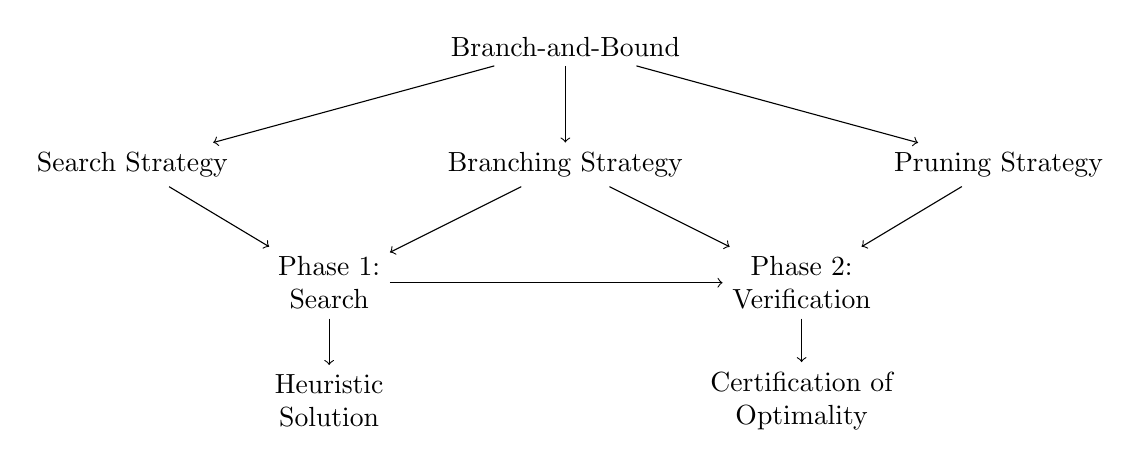
\begin{tikzpicture}[node distance=1.5cm]
                    \node (bb) {Branch-and-Bound};
                    \node (Branching) [below of=bb] {Branching Strategy};
                    \node (Select) [right of=Branching, xshift = -7cm] {Search Strategy};
                    \node (Pruning) [left of=Branching, xshift = 7cm] {Pruning Strategy};
                    \node (Search) [below of=Branching, xshift = -3cm, align=center] {Phase 1:\\Search};
                    \node (Verification) [below of=Branching, xshift = 3cm, align=center] {Phase 2:\\Verification};
                    \node (heu) [below of=Search, align=center] {Heuristic\\Solution};
                    \node (cer) [below of=Verification, align=center] {Certification of\\Optimality};
                    \draw [->] (bb) -- (Select);
                    \draw [->] (bb) -- (Branching);
                    \draw [->] (bb) -- (Pruning);
                    \draw [->] (Select) -- (Search);
                    \draw [->] (Branching) -- (Search);
                    \draw [->] (Branching) -- (Verification);
                    \draw [->] (Pruning) -- (Verification);
                    \draw [->] (Search) -- (Verification);
                    \draw [->] (Search) -- (heu);
                    \draw [->] (Verification) -- (cer);
                \end{tikzpicture}
            \end{figure}

        \subsection{Search Strategy: Choose Node to Branch}
            \paragraph{Depth-first search}
                It can be implemented by maintaining the list of unexplored subproblems $L$ as a stack. The algorithm removes the top item from the stack to choose the next subproblem to explore, and when children are generated as a result of branching, they are inserted on the top of $L$. Thus, the next subproblem that is explored is the most recently generated subproblem.

                \begin{itemize}
                    \item DFS does not need to store the entire list of unexplored subproblems (only stores the path from the root of T to the current subproblem)
                    \item If no unexplored children remain, the algorithm backtracks to the closest ancestor node with unexplored children.
                    \item Use the LP relaxations as lower bounds. The LP solver can often reuse information from the parent LP solution as a starting point for the child LP solution
                    \item Naive implementations of DFS do not use any information about problem structure or bounds
                    \item Search tree is extremely unbalanced
                \end{itemize}

            \paragraph{Breadth-first search}
                BFS explores all subproblems that are at a fixed distance from the root before exploring any deeper subproblems.

                \begin{itemize}
                    \item Finding an optimal solution that is closest to the root of the tree, thus operating well on unbalanced search trees
                    \item Generally unable to exploit pruning rules that compare against the current incumbent solution $\Rightarrow$ high memory
                    \item Best bound search $\Rightarrow$ improve dual bound
                    \item Best estimate search $\Rightarrow$ improve primal bound
                \end{itemize}

            \paragraph{Best-first search, A* search}
                makes use of a heuristic measure-of-best function to compute every subproblem by a admissible index $\mu$.

        \subsection{Branching Strategy: Choose Branching Variable}
            % \paragraph{The goal of Branching}
            %     \begin{itemize}
            %         \item Divide the problem into easier subproblems
            %         \item We want to chose the branching variables that minimize the sum of the solution times of the sub-problems
            %         \item If after branching the $u(S_i)$ changes a lot,
            %         \begin{itemize}
            %             \item we can find a good L first
            %             \item the branch may get worse than the current bound first
            %         \end{itemize}
            %         \item Instead of solving the potential two branches for all candidates to optimality, solve a few iterations of the dual simplex, each iteration of pivoting yields an upper bound.
            %     \end{itemize}
                
            \paragraph{The Most Violated Integrality constraint}
                Pick the $j$ of which $x_j - \lfloor \hat{x_j} \rfloor$ is the closest to 0.5

            \paragraph{Strong Branching}
                Select a few candidates $(K)$, create sub-problems for each of these variables, run a few dual simplex iterations to see the improved bounds, select the variable with the best bounds, and then selects for branching the variable that induces the most change in the objective.

                \begin{itemize}
                    \item Might fix variable, when one side is infeasible
                    \item Detect infeasibility, when both side are infeasible
                    \item Can be speed up by limit the number of iterations, or stop when improvement is found.
                    \item Domain propagation
                \end{itemize}

            \paragraph{Pseudo-cost Branching}               
                
                Pseudo-cost attempts to predict the per-unit change in the objective function for each candidate branching variable, based on past experience in the tree. The basic idea of this strategy is to keep track for each variable $x_i$ the change in the objective function when this variable was previously chosen as the variable to branch on. By branching on a variable that is expected to produce a significant change in the objective function, it is more likely that the generated subproblems can be pruned. One difficulty with pseudocost branching is that no information about past branching behavior is available at the beginning of the algorithm, so the pseudocosts for each variable must be initialized in some way.

                For variable $x_j\in K$, 
                
                \begin{equation*}\begin{cases}P_j^+, & \text{bound reduction if rounded up} \\ P_j^-, & \text{bound reduction if rounded down}\end{cases}\end{equation*}

                define $f_j = x_j -\lfloor x_j \rfloor$
                \begin{equation*}\begin{cases}D_j^+ = P_j^+ (1-f_j) \\ D_j^- = P_j^- f_j\end{cases}\end{equation*}

                \begin{figure}[H]
                    \centering
                    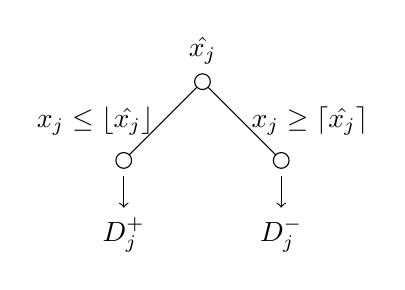
\begin{tikzpicture}[scale=0.2]
                        \draw (0, 5) circle [radius=0.5];
                        \draw (-5, 0) circle [radius=0.5];
                        \draw (5, 0) circle [radius=0.5];
                        \draw (0.353, 4.647) -- (4.647, 0.353);
                        \draw (-0.353, 4.647) -- (-4.647, 0.353);
                        \node [above] at (0, 5.5) {$\hat{x_j}$};
                        \node [left] at (-2.5, 2.5) {$x_j \le \lfloor \hat{x_j} \rfloor$};
                        \node [right] at (2.5, 2.5) {$x_j \ge \lceil \hat{x_j} \rceil$};
                        \draw [->] (-5, -1) -- (-5, -3);
                        \draw [->] (5, -1) -- (5, -3);
                        \node [below] at (-5, -3) {$D_j^+$};
                        \node [below] at (5, -3) {$D_j^-$};
                    \end{tikzpicture}
                    \caption{Strong Branching}
                \end{figure}

                For those variables in $K$ find the
                \begin{itemize}
                    \item $\max \{\min\{ {D_j^+},  {D_j^-}\}\}$, or
                    \item $\max \{\max\{ {D_j^+},  {D_j^-}\}\}$, or
                    \item $\max \{\frac{D_j^+ + D_j^-}{2}\}$, or
                    \item $\max \{\alpha_1\min\{ {D_j^+},  {D_j^-}\} + \alpha_2\max\{ {D_j^+},  {D_j^-}\}\}$
                \end{itemize}
                
                to branch.

        \subsection{Branching Strategy: Create Offspring}

            \paragraph{Traditional Branching}
                For $\hat{x} \notin S$, $\exists j \in N$ such that

                \begin{equation*}\hat{x_j} -\lfloor\hat{x_j}\rfloor > 0 \end{equation*}

                Create two sub-problems

                \begin{figure}[H]
                    \centering
                    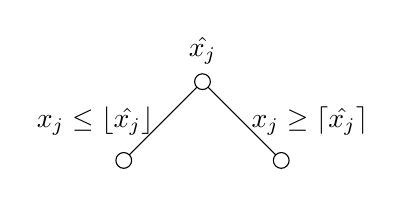
\begin{tikzpicture}[scale=0.2]
                        \draw (0, 5) circle [radius=0.5];
                        \draw (-5, 0) circle [radius=0.5];
                        \draw (5, 0) circle [radius=0.5];
                        \draw (0.353, 4.647) -- (4.647, 0.353);
                        \draw (-0.353, 4.647) -- (-4.647, 0.353);
                        \node [above] at (0, 5.5) {$\hat{x_j}$};
                        \node [left] at (-2.5, 2.5) {$x_j \le \lfloor \hat{x_j} \rfloor$};
                        \node [right] at (2.5, 2.5) {$x_j \ge \lceil \hat{x_j} \rceil$};
                    \end{tikzpicture}
                    \caption{Traditional Branching}
                \end{figure}

            \paragraph{Constraint Branching}

                Use parallel constraints to branch, e.g.

                \begin{figure}[H]
                    \centering
                    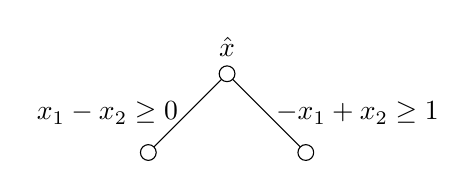
\begin{tikzpicture}[scale=0.2]
                        \draw (0, 5) circle [radius=0.5];
                        \draw (-5, 0) circle [radius=0.5];
                        \draw (5, 0) circle [radius=0.5];
                        \draw (0.353, 4.647) -- (4.647, 0.353);
                        \draw (-0.353, 4.647) -- (-4.647, 0.353);
                        \node [above] at (0, 5.5) {$\hat{x}$};
                        \node [left] at (-2.5, 2.5) {$x_1 - x_2 \ge 0$};
                        \node [right] at (2.5, 2.5) {$-x_1 + x_2 \ge 1$};
                    \end{tikzpicture}
                    \caption{Constraint Branching}
                \end{figure}
            
            \paragraph{Special Ordered Sets of type 1 (SOS1 or S1)} are a set of variables, at most one of which can take a non-zero value, all others being at 0. 

                \begin{figure}[H]
                    \centering
                    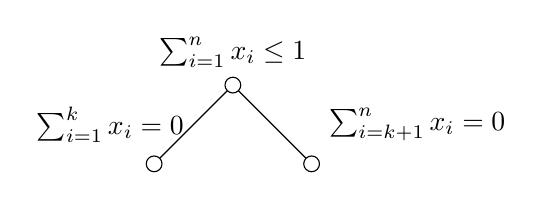
\begin{tikzpicture}[scale=0.2]
                        \draw (0, 5) circle [radius=0.5];
                        \draw (-5, 0) circle [radius=0.5];
                        \draw (5, 0) circle [radius=0.5];
                        \draw (0.353, 4.647) -- (4.647, 0.353);
                        \draw (-0.353, 4.647) -- (-4.647, 0.353);
                        \node [above] at (0, 5.5) {$\sum_{i=1}^{n}x_i\le 1$};
                        \node [left] at (-2.5, 2.5) {$\sum_{i=1}^{k}x_i=0$};
                        \node [right] at (5.5, 2.5) {$\sum_{i=k+1}^{n}x_i=0$};
                    \end{tikzpicture}
                    \caption{SOS1 Branching}
                \end{figure}

            \paragraph{Special Ordered Sets of type 2 (SOS2 or S2)}: an ordered set of non-negative variables, of which at most two can be non-zero, and if two are non-zero these must be consecutive in their ordering. 

                \begin{figure}[H]
                    \centering
                    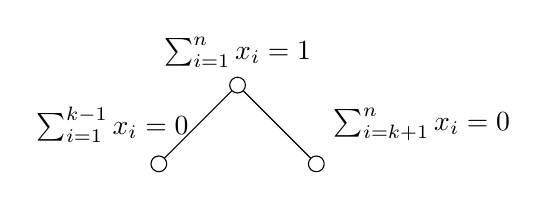
\begin{tikzpicture}[scale=0.2]
                        \draw (0, 5) circle [radius=0.5];
                        \draw (-5, 0) circle [radius=0.5];
                        \draw (5, 0) circle [radius=0.5];
                        \draw (0.353, 4.647) -- (4.647, 0.353);
                        \draw (-0.353, 4.647) -- (-4.647, 0.353);
                        \node [above] at (0, 5.5) {$\sum_{i=1}^{n}x_i = 1$};
                        \node [left] at (-2.5, 2.5) {$\sum_{i=1}^{k-1}x_i = 0$};
                        \node [right] at (5.5, 2.5) {$\sum_{i=k+1}^{n}x_i = 0$};
                    \end{tikzpicture}
                    \caption{SOS2 Branching}
                \end{figure}
                      
            \paragraph{Ryan-Foster}
                Ryan-Foster is for Set covering problem. The typical model is
                \begin{align*}
                    \text{min} \quad & \sum_{i \in C} x_i \\
                    \text{s.t.} \quad & \sum_{i \in C} a_{ij}x_{i} \ge 1, \quad \forall j \in U \\
                            & x_i \in \{0, 1\}, \quad \forall i \in C 
                \end{align*}
                For any fractional solution, there are at least two elements $(i,j)$ so that $i$ and $j$ are both partially covered by the same set $S$, but there is another set $T$ that only covers $i$
                
                \begin{figure}[H]
                    \centering
                    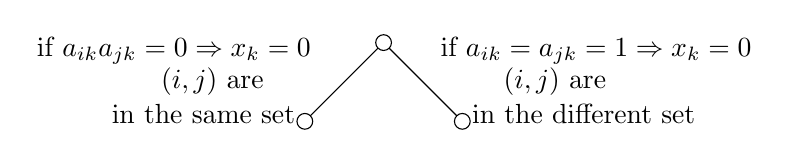
\begin{tikzpicture}[scale=0.2]
                        \draw (0, 5) circle [radius=0.5];
                        \draw (-5, 0) circle [radius=0.5];
                        \draw (5, 0) circle [radius=0.5];
                        \draw (0.353, 4.647) -- (4.647, 0.353);
                        \draw (-0.353, 4.647) -- (-4.647, 0.353);
                        \node [left] at (-7, 2.5) {$(i,j)$ are};
                        \node [left] at (-5, 0.5) { in the same set};
                        \node [left] at (-4, 4.5) {if $a_{ik}a_{jk}=0 \Rightarrow x_k = 0$};
                        \node [right] at (7, 2.5) {$(i,j)$ are};
                        \node [right] at (5, 0.5) { in the different set};
                        \node [right] at (3, 4.5) {if $a_{ik}=a_{jk}=1 \Rightarrow x_k=0$};
                    \end{tikzpicture}
                    \caption{Ryan Foster Branching}
                \end{figure}

        \subsection{Pruning Rules}
            \paragraph{Lower bound}
                The most common way to prune is to produce a lower bound on the objective function value at each subproblem, and use this to prune subproblems whose lower bound is no better than the incumbent’s solution value. Lower bounds are computed by relaxing various aspects of the problem.

                \begin{itemize}
                    \item Many different lower bound can be computed
                    \item Attempt to prune using the easy lower bounds first, then move on to more complex
                    \item One of the ``easy lower bound'' can be LP relaxation
                    \item Another ``easy lower bound'' can be Lagrangian relaxation for IP.
                \end{itemize}

            \paragraph{Dominance relations}
                In contrast to lower bounding rules, dominance relations allow subproblems to be pruned if they can be shown to be dominated by some other subproblem. In other words, if subproblem $S_1$ dominates subproblem $S_2$ , this means that for any solution that is a descendant of $S_2$ , there exists a complete solution descending from $S_1$ that is at least as good. 

    \section{*Use Branch-and-Bound to Solve Other Problems}
        \paragraph{Close-enough Traveling Salesman Problem}
            Given a set of vertices $V = \{0, 1, \cdots, n\}$ in a 2-dimensional space with coordinates $(\bar{x}, \bar{y}), i = 0, 1, \cdots, n$. Each vertex $i$ is in the center of a convex region bounded by a circle $D_i$ with radius $r_i$. Assume that $(\bar{x}_i, \bar{y}_i) \neq (\bar{x}_j, \bar{y}_j), \forall i, j \in V, i \neq j$. The problem lies in determining the value of the coordinates of the hitting points $(\bar{x}_i, \bar{y}_i) \in \mathbb{R}^2$ and a sequence $L = (k_0, k_1, \cdots, k_n), k_i \in V$ representing the order in which the vertices are covered, such that the tour over the hitting points forms a Hamiltionian cycle of minimum length and $(\bar{x}_i, \bar{y}_i) \in D_i, i \in V$.

        \paragraph{Coutinho et al. 2016} Each branch-and-bound node is associated with an optimal partial tour that needs to visit only a given subset of vertices in a particular order. At the root node, the algorithm chooses three vertices to generate an initial sequence of nodes that need to be visited. Because there are only three vertices involved in this sequence and costs are symmetric, their order will not affect the solution. Therefore, the problem of finding an optimal tour that visits these three vertices in the given order is a valid relaxation of the main problem regardless of the choice of the initial sequence. If the associated solution is feasible, i.e., all customers are covered, then this solution is optimal and the problem is solved. Otherwise, for this root node, the algorithm branches into three subproblems; in each of them, a vertex that does not belong to the tour is inserted in a different position. A node is discarded if its cost is greater than or equal to the best known upper bound or if its associated solution is feasible. Otherwise, a branching is performed over this node using the same rationale applied in the root node. Note that the number of child nodes (subproblems) for every node in the tree is equal to the number of vertices in the partial sequence of the parent node. \citep{Coutinho2016}

        \begin{figure}[H]
            \centering
            \includegraphics[width=1\textwidth]{../../image/BnB_CETSP.png}
            \caption{An example of the B\&B algorithm for an instance with 7 vertices}
            \label{fig:BnB_CETSP}
        \end{figure}

    \bibliography{literature}
\end{document}